\chapter{GUI Startup}
\label{s:gui.startup}

%--------------------------------------------------------------
\section{Starting the GUI}

The GUI can be started from the system shell by executing the command
\begin{example}
  python -m pytao.gui
\end{example}
You can also specify any of the command line options that \tao supports.  For example,
\begin{example}
  python -m pytao.gui -init_file ~/bmad_dist/tao/examples/cesr/tao.init -rf_on
\end{example}
This will prefill the settings for \texttt{init_file} and \texttt{rf_on}. The GUI starts with the
window shown in Figure \ref{fig:startup}. From here, all of the command-line settings that Tao
supports can be set (settings that are left blank are omitted when Tao is started). The parameters
above the horizontal separator bar are \tao parameters and the parameters below the bar are GUI
specific parameters.

Towards the bottom of the window, below the horizontal separator, are some settings that are
specific to the GUI.  The "Interface to Tao" setting controls whether the \vn{ctypes} or
\vn{pexpect} backend for communicating with Tao will be used.  Below it, the "Shared Library" (if
"Interface to Tao" is set to "ctypes") or "Tao Executable" (if "Interface to Tao" is set to
"pexpect") setting points the GUI to the correct executable or shared object library to use.  In
most cases, the GUI will prefill this box by referencing the ACC_LOCAL_ROOT and ACC_ROOT_DIR
environmental variables.

The setting of \vn{Plot Mode} controls what plotting environment is used. Possible setting are:
\begin{example}
  matplotlib
  pgplot/plplot
  none
\end{example}
\vn{MatPlotLib} is a python based package which is the most versatile. The \vn{pgplot/pgplot} option
is the standard tao plotting used with the command line version of \tao. Note: Which plotting package is
used with \vn{pgplot/plplot}, either \vn{pgplot} or \vn{plplot}, is determined by how \tao was compiled.

Finally, the font size can be set as desired. Hitting Enter/Return while the font size box is in
focus will adjust the font size of the startup window to give the user a sense of what the chosen
font size will look like.

Once all of the startup settings have been set, clicking "Start Tao" will initialize Tao and bring
the user to the main GUI window.

\begin{figure}
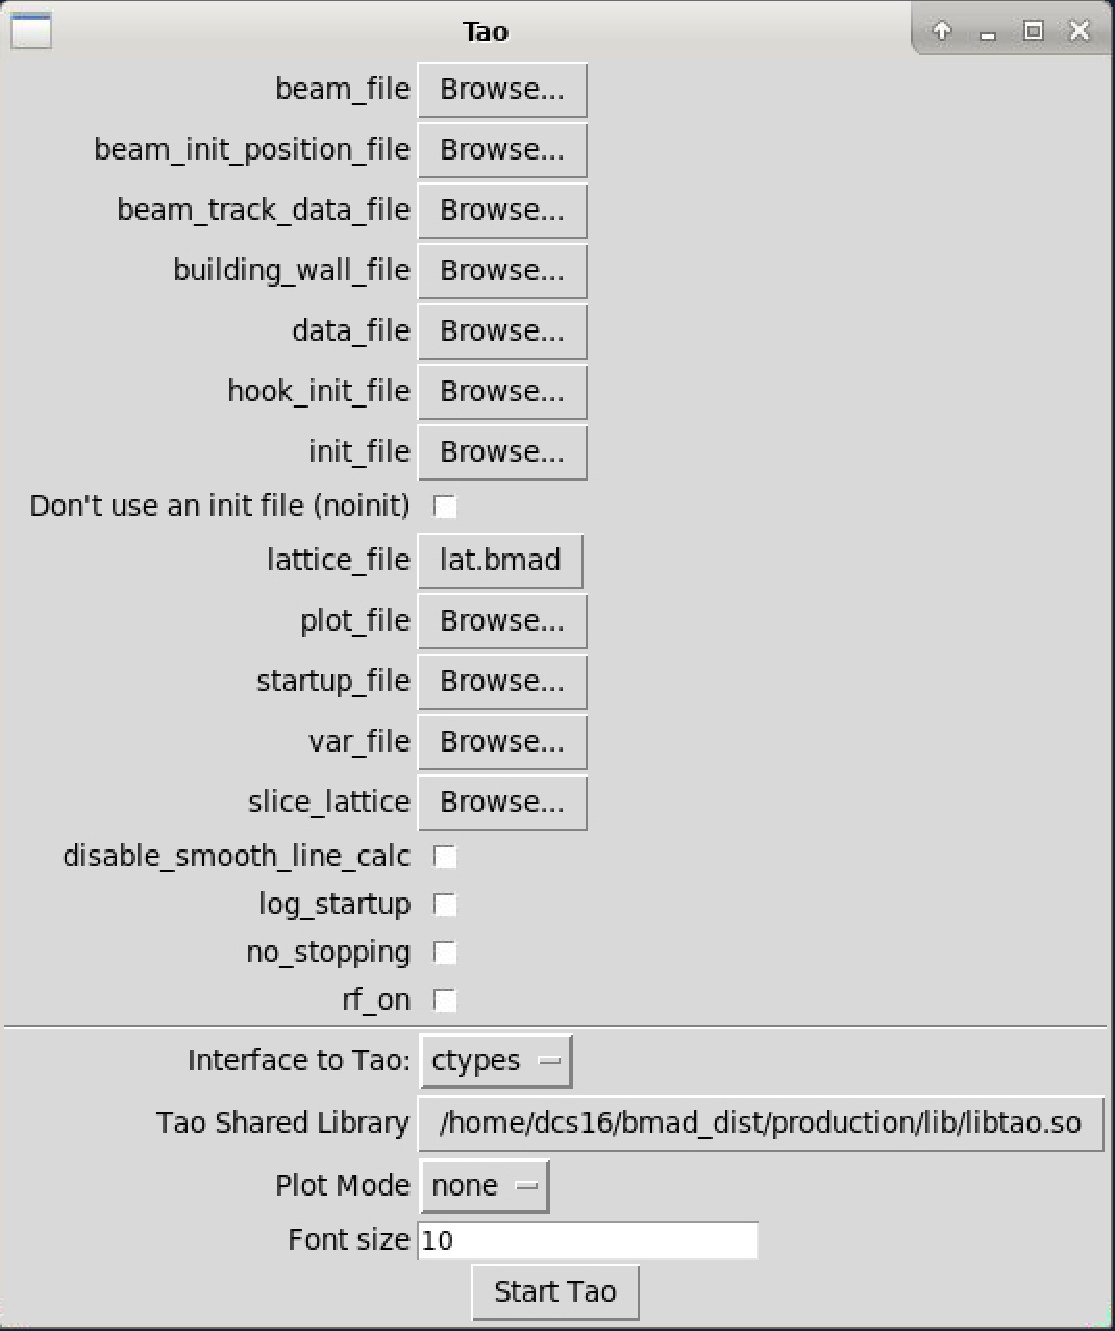
\includegraphics[width=8cm]{figures/startup.pdf}
\centering
\caption[The GUI startup window.]{The GUI startup window. In this example, the init file that tao should use has been specified.}
\label{fig:startup}
\end{figure}

%--------------------------------------------------------------
\section{GUI Initialization File}
\label{s:gui.init.file}

To speed up the initialization process, you can make an init file for the GUI.  This file should be called "gui.init", and it should be in the same directory from which you start the GUI.

gui.init should have each option on a separate line, and each option should be listed in the form "parameter:value".  For example, the text below would constitute a good gui.init file:
\begin{example}
  #MY GUI INIT FILE
  beam_file:/path/to/beam/file
  data_file:/path/to/data/file
  #THIS IS A COMMENT
  disable_smooth_line_calc:T
  rf_on:T
  tao_executable:/path/to/executable
\end{example}
For \tao specific parameters, the names in the \vn{gui.init} file correspond to the names in the startup window
(\fig{fig:startup}) or in one case, the name in parentheses. For GUI specific parameters (below the horizontal separator), replace blanks between words and
make all letters lower case. For example, ``\vn{Interface to Tao}'' in the startup window becomes \vn{interface_to_tao}
in the \vn{gui.init} file. Note: The startup window can be bypassed altogether by setting \vn{start_tao} in \vn{gui.init}
to \vn{True}.

The order in which you list options in gui.init is not important.

File paths should be specified in full to be safe, but you can specify paths relative to the directory from which you launch main.py.  For example, "/home/username/file", "subfolder/my_file", and "../../path/to/another/file" would all be acceptable file paths.  You can also use your environmental variables and "\textasciitilde{}", as in "\textasciitilde{}/Documents/my_file" and "\$DIST_BASE_DIR/tao/file".

For logical parameters, for example, "rf_on", Use T/F or True/False as the parameter's value.

You can also include comments with \#.  Anything after a \# character will be ignored.

To get a list of parameters that can be set in a \vn{gui.init} file, start Tao with the command
\begin{example}
  tao -help
\end{example}
The corresponding gui.init parameter is the Tao parameter with the leading dash "-" removed and a
colon ":" between the parameter and the parameter's value. 

